\documentclass[border={-4pt -6pt -4pt -4pt}]{standalone}

\usepackage{hyperref}
\usepackage{tikz}

\usetikzlibrary{decorations.pathreplacing,
  arrows,
  calc,
  decorations.pathmorphing,
  decorations.pathreplacing,
  decorations.markings,
  positioning,
  shapes
}

\ifpdf
% Ensure reproducible output
\pdfinfoomitdate=1
\pdfsuppressptexinfo=-1
\pdftrailerid{}
\hypersetup{
  pdfcreator={},
  pdfproducer={}
}
\fi

\begin{document}
\begin{tikzpicture}
  \node at (0.0, 0) {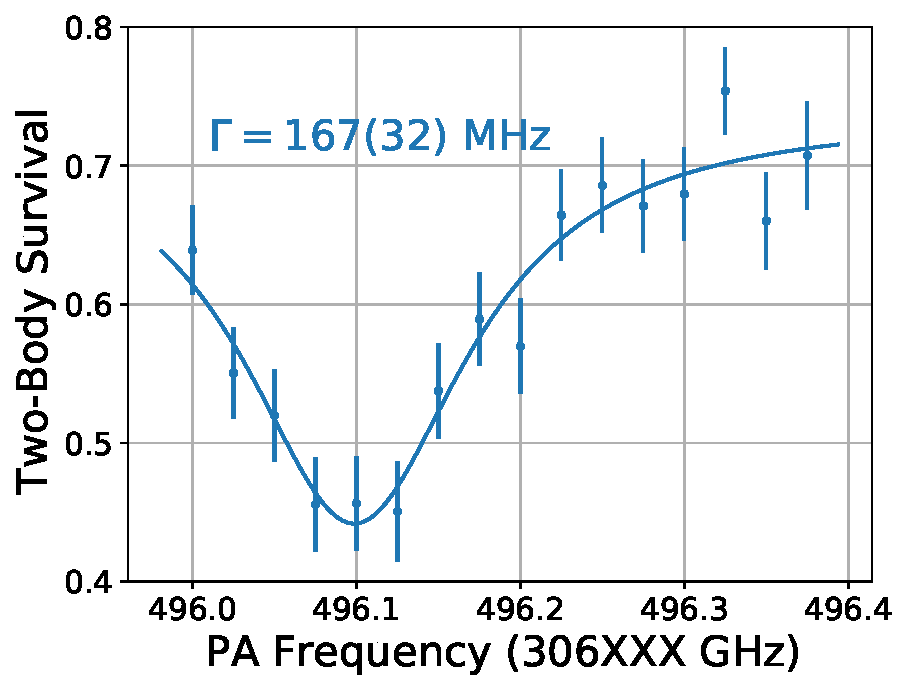
\includegraphics[height=4.5cm]{pa_spectrum_v12_red_10.pdf}};
  \node at (-1.8, 1.89) {\scriptsize (\textbf{A})};
  \node at (6, -0.05) {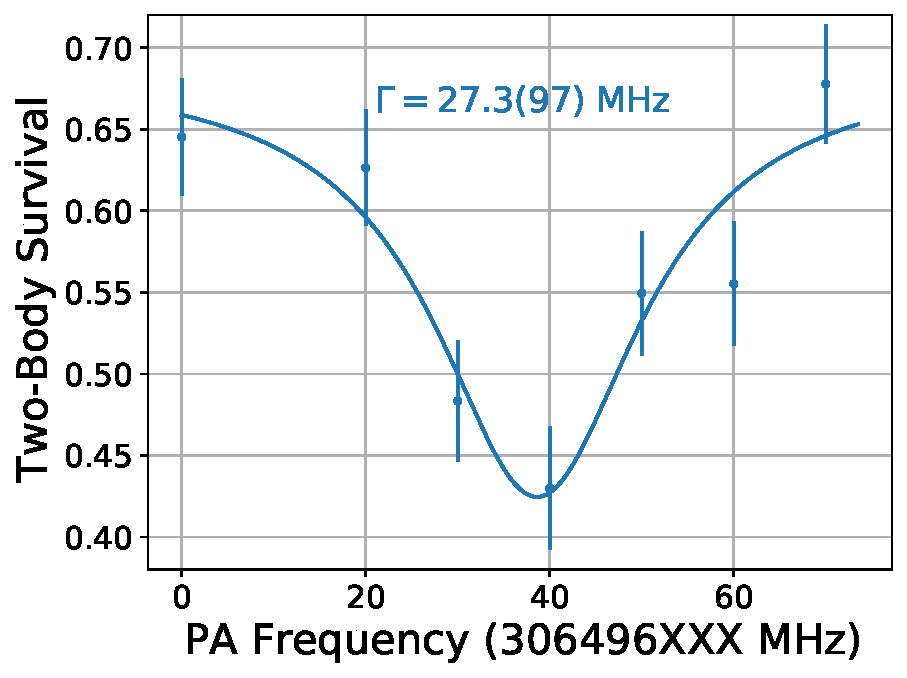
\includegraphics[height=4.5cm]{pa_spectrum_v12_red_1.pdf}};
  \node at (4.3, 1.9) {\scriptsize (\textbf{B})};
  \node at (3, -4.6) {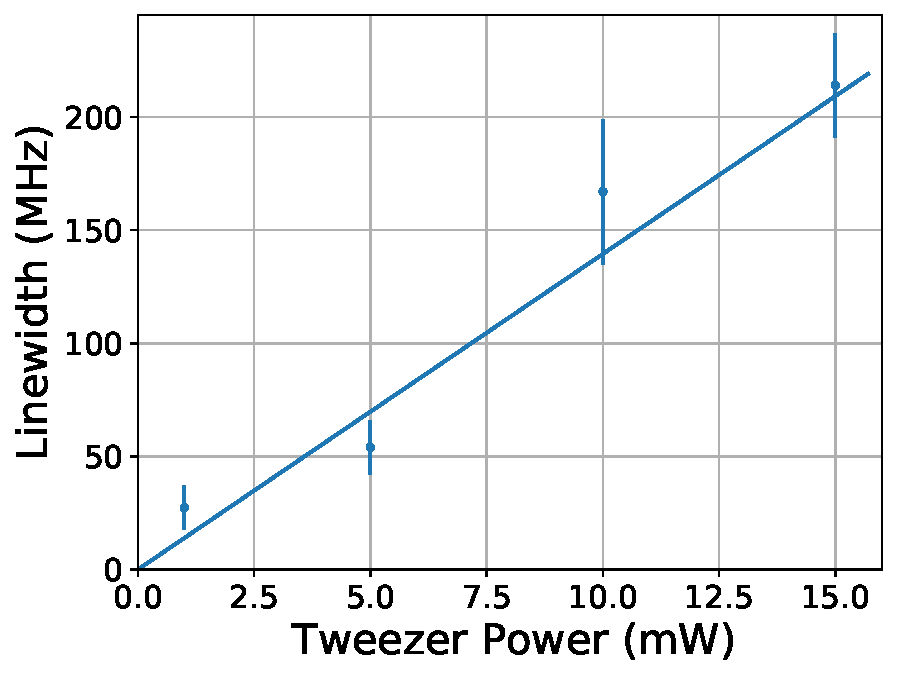
\includegraphics[height=4.5cm]{pa_linewidth_tw_pwr.pdf}};
  \node at (1.3, -2.65) {\scriptsize (\textbf{C})};
\end{tikzpicture}
\end{document}
